\section{Durchführung}
\label{sec:Durchführung}

\subsection{Aufnahme des Röntgenspektrums}

Es wird eine evakuierte Röhre mit Glühkathode und einer Kupferanode so ausgerichtet, dass die Röntgenstrahlen auf einen Lithiumfluorid-Kristall treffen.
Der LiF-Kristall ist drehbar, sodass eine Reihe von Winkeln eingestellt werden können.
Zuletzt wird ein Geiger-Müller-Zählrohr hinter dem LiF-Kristall angebracht, um die Impulse bei unterschiedlichen Kristallwinkeln messen zu können.
Nun werden in Abschnitten von $\Delta \alpha = 0.1°$ bei einer Integrationszeit von $t = 10s$ und einer Beschleunigungsspannung von $U = 35kV$ die Impulse des Geiger-Müller-Zählrohrs gemessen.
Der Winkel wird von $8°$ bis $25°$ eingestellt.

\subsection{Bestimmung der Transmission}

Für die Bestimmung der Transmission wird ein Aluminium-Absorber verwendet.
Es müssen 2 Messungen durchgeführt werden, eine mit und eine ohne Absorber.
Die Winkel sind von $7°\ -\ 10°$ einzustellen, in Abschnitten von $\Delta \alpha = 0.1°$.
Die Integrationszeit beträgt $t = 200s$, bei einer Beschleunigungsspannung von $U = 35kV$.
Zuerst soll eine Totzeitkorrektur berechnet werden, dann sollen die neuen Werte in einem $T(\lambda)$-Diagramm dargestellt werden.

\subsection{Bestimmung der Compton-Wellenlänge}

Um die Compton-Wellenlänge zu bestimmen, wird der Versuch, wie in \autoref{fig:aufbau} dargestellt, umgebaut.
Der LiF-Kristall wird durch ein Plexiglasstreuer ersetzt.
Es müssen drei Messungen vorgenommen werden: Einmal ohne Absorber, einmal zwischen Röntgenstrahler und Streuer und einmal zwischen Streuer und Zählrohr.
Die Integrationszeit soll $t = 300s$, bei einer Spannung von $U = 35kV$, betragen.
Aus den Messdaten sollen die Transmissionen berechnet werden und aus diesen ihre äquivalente Wellenlängen.
Die Differenz der Wellenlänge ist die Compton-Wellenlänge.

\begin{figure}[htbp]
    \centering
    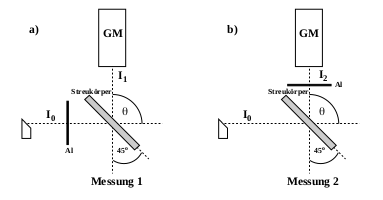
\includegraphics{content/Aufbau_Compton.png}
    \caption{Umbau für die Bestimmung der Compton-Wellenlänge. In $a)$ sitzt der Absorber zwischen Strahler und Streuer, in $b)$ zwischen Streuer und Zähler.}
    \label{fig:aufbau}
\end{figure}